\chapter{Embedded Code Service and Python Scanner}

In this chapter we follow up on the Manta Flow platform description and explain the problem of analysing embedded code in this context. We analyze multiple technologies that support embedded code and formulate our requirements for the solution. Then we analyze how to integrate embedded code analysis into scanners and finally, we analyze AWS Glue as a proof-of-concept technology for embedded code analysis.

Embedded code service is responsible for analyzing data lineage in code embedded in various technologies and merging its lineage graph to that of the source technology. Similarly to query service, it enables merging of data lineage of two cooperating technologies into one graph utilizing the existence of separate scanners for each of the respective technologies. It provides a way to compose a more complete lineage for the given technology without the need to implement the specifics of analyzing the embedded code within the source technology scanner.

%%----- SECTION -----%% 
\section{Embedded code service analysis}

There are multiple problems that embedded code service needs to address. Here is the list for an overview:
\begin{enumerate}
    \item Multiple supported languages (Python, Java, C\#)
    \item Merging embedded code graph to the enclosing technology graph
    \item Specifying runtime configuration - available libraries etc.
    \item Running the scanner for the embedded code without Manta Flow hooks
    \item Configuration of individual embedded code service components
    \item Input for Bytecode and C\# - embedded code is in plain text but these scanners expect compiled intermediate code on input, C\# can somehow compile it but Java can’t
    \item Caching
\end{enumerate}
Let’s now take a closer look at each of the problems.

\subsection{Multiple supported languages}
Embedded code service should be a universal service for all programming languages supported in MANTA Flow. A common service enables code reuse as multiple parts of the problem will be solved in a similar way regardless of used programming language and technology. While some approaches may be common on a programming language level (e.g., processing of Java code will include similar steps across all technologies), we can also find similarities between the technologies too (e.g., procedures written in embedded code in databases regardless of the programming language used). Additionally, some steps are common for any combination of technology and programming language, such as merging the graphs of embedded code and parent technology.
\par
Providing a common service for all languages brings in additional complexity that needs to be addressed. Each technology and programming language has its specifics, so the service needs to be highly configurable to facilitate these differences. We can find inspiration in the already mentioned query service design. This service uses dialect specification to deal with different dialects of data query languages. 
\par
In our case, dialects are not a problem, in general, Bytecode is always Bytecode, Python is always Python. One could argue that there is Scala and Java or their different versions, Python and IPython etc. However, dealing with these dialects is solved by the language scanners themselves and does not need to be covered any further than providing the information about which language (and its version) is used.
\par
A more important problem for programming languages is “orchestration”. All current programing languages use some form of import mechanism where the developers can import additional libraries and frameworks. This is also the case for the embedded code, often there is a mechanism of adding external libraries to be imported by the embedded code. This is, however, not as straight-forward as in applications written entirely in that programming language. Some technologies perform additional orchestration to run the embedded code correctly, such as injecting it in a well-defined class, so the envelope does not have to be written by the user every time, adding the desired imports and only then the code is run on the execution engine used by that technology. This process has to be mimicked by embedded code service before analyzing the code by the language scanner to provide a functional code that can be analyzed.
\par
The orchestration would generally be different for each technology and programming language with repeating patterns, so the interface of the embedded code service should allow specification of these process individually with the ability to reuse the already implemented patterns.

\subsection{Merging embedded code graph to the enclosing technology graph}
Sometimes, embedded code can be connected with the enclosing technology to parameterize the execution of the embedded code (e.g., passing filtering arguments to a database procedure). Often this is done by reading a specific variable or property provided by the enclosing technology. These values could be a part of the data lineage and it would be great if they could be propagated towards the lineage of the embedded code and merged together so they create a single lineage graph. 
\par
Merging these graphs is not a trivial task, so it would be best if it was handled by the embedded code service, so developers of other scanners are shielded from its specifics. While the developer knows what they want to connect, they don’t need to know how to connect it, they just use the embedded code service interface. This is similar to what query service offers. This interface can be very similar to that of query service and even some code base could be reused (it requires a further, deeper analysis). 

\subsection{Specifying runtime configuration}
As we already mentioned, often the runtime configuration of embedded code can be configured in the enclosing technology and it then orchestrates the runtime where the embedded code is executed. The embedded code then omits this information, it is just pure code. In addition to libraries loaded from the file system, it is often possible to just specify the names and versions of desired libraries and the enclosing technology prepares these libraries using some package manager, e.g., pip in Python. In such case, the source code of the libraries is not available for analysis.
\par
Additionally, currently existing language scanners are designed to work with extracted source code/intermediate language. To facilitate dynamic runtime configurations, their interface needs to be modified so that it is possible to pass the information about the desired runtime even when the entire source code is not available. This is mainly important for the Python scanner which is currently dependent on receiving all source code.
\par
In general, it is difficult to estimate what properties need to be passed about runtime configuration for all technologies and languages. However, we don’t need to specify that in a general way. This information is only relevant for the parent technology where it is known what can and needs to be provided and the implementation of embedded code service for that particular language, which needs to prepare the input based on the configuration. Therefore, the configuration contract only needs to exist between these two components and all other components only need to read the source technology and the target programming language, so the contract can be highly customizable. Using polymorphism for runtime configuration seems like a good choice as it can provide both a type-safe and customizable interface.

\subsection{Running the scanner for the embedded code without Manta Flow hooks}
Similarly to the previous problem, this also involves the interface of programming language scanners. These are currently designed to be started by a Manta Flow scenario, responding to hooks. It is desired to modify this interface to enable starting the scanners from embedded code service. These modifications should not be big (the scanners are already quite well designed), but it is important to keep in mind that they need to be finished before a language scanner can be added to the embedded code service. 

\subsection{Configuration of individual embedded code service components}
The process of analyzing code consists of multiple steps, each performed by an individual component. First, there is input orchestration, then input analysis by Reader component and lastly, generating Manta Flow graph from intermediate language graph. So far, all language scanners use common dataflow generator. This could change for future languages, but so far all of them use it.
\par
To make all of this work, these components need to be correctly configured. Currently, the interaction between reader and dataflow generator is facilitated by Spring beans. There will also need to be new <language>EmbeddedCodeService components added for each scanner that implement the embedded code service interface for that particular language. These sub-components will then be injected to the EmbeddedCodeService component that will be available to other technology scanners using Spring. There are two possible ways to configure these sub-components:
\begin{enumerate}
    \item self-contained component that packages orchestration, reader and dataflow generator and implements a required interface, common parts can be implemented by an abstract superclass
        \begin{figure}[ht]\centering
        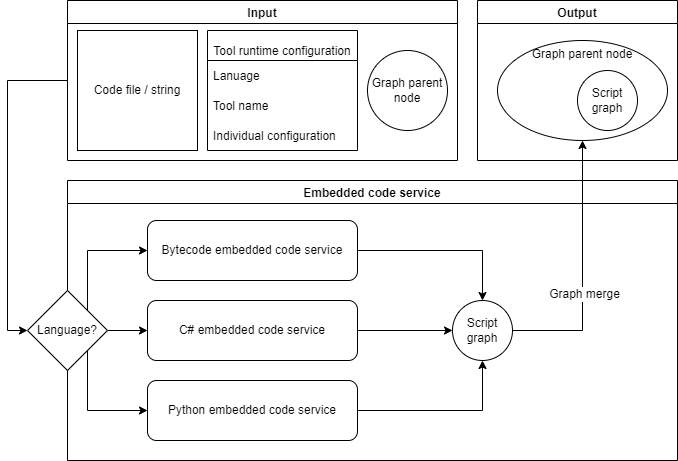
\includegraphics[width=1.0\textwidth]{img/Embedded code service base design 1.png}
        \caption{Option 1}
        \label{fig01:ECSbasedesign01}
        \end{figure}    
    \item a component that only handles orchestration and input preparation and then EmbeddedCodeService will pass the input to its own instances of reader and dataflow generator using well-defined interfaces
        \begin{figure}[ht]\centering
        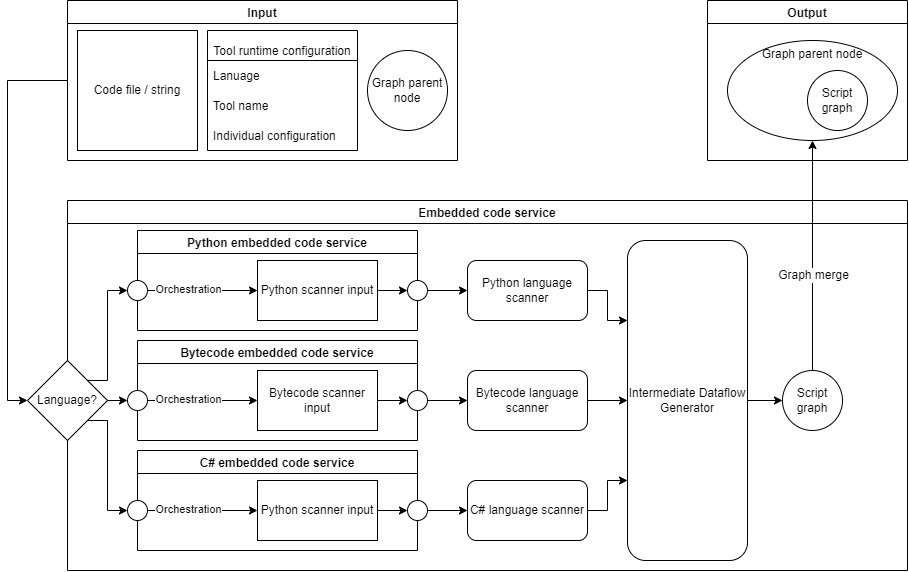
\includegraphics[width=1.0\textwidth]{img/Embedded code service base design 2.png}
        \caption{Option 2}
        \label{fig01:ECSbasedesign02}
        \end{figure}    
\end{enumerate}

The preferred option is the first one as it enables each language scanner to have a slightly different interface. This interface only needs to satisfy the needs of <language>EmbeddedCodeService component for that language. The scanners and languages differ in many details, this approach would provide some maneuvering space. The second option would allow the individual <language>EmbeddedCodeServices to be more lightweight since their only executive role is to perform orchestration, but would enforce strict interfaces for the language scanners.

\subsection{Input for Bytecode and C\#}
Usually, embedded code is available in plain text but Bytecode and C\# scanners expect compiled intermediate code on input. Currently, C\# scanner can compile the code itself, although it has some limitations. Bytecode scanners lacks this functionality entirely, so it would have to be added. 
\par
A prerequisite for a successful compilation is presence of all dependencies. That could prove to be a bigger problem than compilation itself as not always all dependencies are available and compiling unknown code can also cause some security issues.
\par
A small workaround could be to compile the embedded code using generated stubs. The compiler only requires the declarations to be available so that the correct call instructions can be generated. Since the scanners only analyze intermediate code, such code would be the same as if it was compiled with the original dependencies and it would be possible to perform the analysis in a standard way. The stubs could be generated using reflection from the original dependencies.
\par
This issue needs to be analyzed further before implementation as it is outside of the scope of this analysis.

\subsection{Caching}
It is also necessary to address the possibility of caching some intermediate data. It can be expected that multiple instances of embedded code can appear during one analysis (multiple scripts within parent technology analysis). These instances have a lot in common. Since they are embedded, they rely on some part of the environment to be provided by the parent technology and this part is often the same. It is therefore valid to consider if some parts can only be computed once and then cached and reused to improve performance.
\par
There is no universal answer and solution for that. There can be some small opportunities in particular cases but no general solutions. However, these particular cases should be reviewed for each language if they can bring some performance benefits.
\par
First opportunity is during input orchestration. As we mentioned earlier, part of the runtime is often the same, so when it is generated and prepared for the first time, it can be stored so it does not need to be generated again. It can be beneficial if this common runtime is considerably large compared to the size of embedded code and the duration of the analysis. For example, currently in Python scanner, parsing standard library which consists of ~2000 files takes longer than performing the analysis of a short script (<100 LOC). In a situation when there are tens or hundreds of such scripts, the improvement could save customer a lot of time. The standard library is available for each script, therefore it could be parsed once and reused. On the other hand, for Bytecode and C\# the input needs to be compiled, so each entry point has to be prepared individually.
\par
The other opportunity is during the analysis. Since we often use the same dependencies, we could maybe cache some intermediate results when analyzing flows in them. However, this optimization is already implemented within the scanners themselves. They use plugins for libraries that mimic the propagation of data flows in library functions and methods, so essentially, no library code is analyzed. Additionally, the execution of the worklist algorithm used for static analysis of the code is highly dependent on the inputs, so it behaves differently for each entry point and therefore there are no shared data between two entry points.
\par
In conclusion, when implementing a new combination of technology-language in embedded code service, it is advised to review the possibility of caching a part of input preparation as it can influence the overall performance of the parent technology.


%%----- SECTION -----%% Analysis of Python scanner w.r.t. Embedded Code service
\section{Python scanner analysis}

Since the Python scanner wasn't initially designed for running embedded code, we need to analyze what are the required changes in order to support Embedded Code Service (further referenced to as ECS).

\subsection{Interface and Spring configuration}
Python Scanner is designed to analyze user inputs. The source code is provided by users and its location together with other settings is provided in scenario configuration. ECS also receives the input, but not the rest of the configuration. This configuration is supposed to be built during its runtime in input orchestration phase of processing embedded code (see DEV-24356: Python embedded code service - Python scanner interface modifications
DONE
). 
\par
Upon analyzing the current state of the components it is clear that they were designed as single-purpose components - they are constructed with all functional elements and task configuration they require. Therefore, the lifecycle of such component ends when it finishes its task as new component has to be constructed for a new task. This is feasible for language scanners running from CLI, because each scenario executes each task once. With ECS the expected lifecycle of components is different. The service is constructed once but can be used for multiple tasks (e.g., analysis of multiple scripts that are a part of one ETL pipeline).
\par
There are two ways how we can modify current components to support both approaches efficiently. Either add a factory for a component that stores the functional elements for its construction and allow passing the configuration as a parameter in a factory method which constructs the component. This approach is suitable for components which hold a complex internal state and it would be costly to refactor it to a stateless component. Also, it is a cheap modification, there are no changes in code, only a factory needs to be added and this change needs to be reflected in Spring configuration.
\par
The other approach is to modify the component to become a stateless component and the task configuration can be passed using dependency injection. This approach is suitable for components that have a single entry-point - a single method that is invoked to complete the task. In such cases the internal state can be kept internally during the execution of the method and thrown away at the end. Alternatively, this state can be passed between the invocations of multiple methods of the component using dependency injection.

\subsection{CLI}
We need to consider one more thing. The components were designed to work with CLI and their interface is customized for that purpose. ECS doesn’t need to implement such interface. Often this interface doesn’t provide exactly the functionality we need and performs additional tasks that are not required (e.g., serializing output to disk). It would be useful to decouple implementation of the functional component from the CLI interface so the functional component can be used by both CLI and ECS but it can have its own interface to perform required tasks.

\subsection{Components}
There are three major components: Extractor, Reader and Dataflow Generator. These are the components that need to be instantiated for both CLI scanner and Embedded Code Service. We therefore need to focus on their interfaces in the scope of this task.

\subsubsection{Extractor}
Extractor almost satisfies our conditions. The configuration is passed to Extractor in constructor, but it is not necessarily needed. It contains some file paths that are read-only and need to be available during extraction. This component can be easily refactored using the first approach. For CLI use-case the configuration is already stored in ExtractorTask that stores both configuration and extractor, so no Spring configuration changes are required.

\subsubsection{Reader}
Reader is a highly state-dependent component. It would require some effort to remove all application-specific information. However, the current implementation requires some refactoring as it does more things than it should. Also, Reader is currently one component that implements CLI interface and performs the tasks. To satisfy all our conditions we need to:
\begin{enumerate}
    \item Decouple CLI interface from the Reader implementation
    \item Identify static sub-components of Reader
    \item Identify task-specific sub-components of Reader
\end{enumerate}
After the refactoring, static sub-components are a part of EntryPointAnalyzer component which can perform the analysis of a single entry point. Task-specific sub-components are a part of AnalyzerConfiguration. This configuration is like a small toolbox that the analyzer uses during the analysis and is provided for each entry point analysis. Lastly, PythonReader component is the implementation of CLI interface and internally uses an EntryPointAnalyzer and its own static AnalyzerConfiguration for its task. 
\par
With these modifications, the Spring configuration needs to be split in two parts. One is general configuration that provides initialized reusable EntryPointAnalyzer. The other is CLI specific that prepares the AnalyzerConfiguration and binds it with PythonReader.

\subsubsection{Dataflow Generator}
Dataflow Generator was reworked during this analysis so we’ll reference only the current implementation after the rework. It was much more simplified and its dependencies were reduced which makes it much easier to use in various contexts. Currently it requires program ID at construction time which is only used during dataflow generation, so it can be easily refactored to be supplied at that time instead and therefore become stateless. It also requires CLI interface decoupling.
\par
After the refactoring, a new DataflowGenerator class is the stateless component of Dataflow Generator. To transform a graph it needs ProgramConfiguration which holds only the program ID, but it is convenient to be a class so it can be instantiated as a bean. Lastly, the TransformationTask is now just the implementation of the CLI interface, previously it represented all of these new components.

\subsubsection{Configuration}
The Spring configuration of Intermediate Dataflow Generator is layered into multiple levels to introduce modularity. This modularity is important as there are currently 3 language scanners that utilize the generator and each of them is slightly different. Moreover, with the introduction of Embedded Code Service, there is another use-case with different needs.  This design reduces the amount of beans that it depends on to a bare minimum and avoids the need to define beans that are unused.
\par
Currently, there are two possible configuration compositions. One is for scanners that are not supported in Embedded Code Service and the other for those that are. For that purpose the configuration of common beans is split in two where the base context configuration sets up the core component of Dataflow Generator that can be used by the service and the context sets up the dataflow task bean that is required for CLI integration. These configurations can then be included in platform specific configuration that provides platform-specific beans.

\subsubsection{Composition without Embedded Code Service}
Without Embedded Code Service the situation is simple as there is only one use-case, so only the platform-specific beans need to be provided.
\begin{figure}[ht]\centering
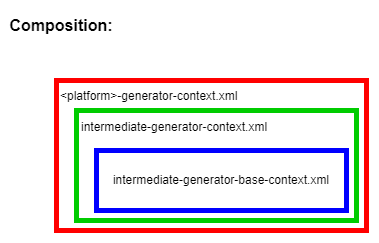
\includegraphics[width=1.0\textwidth]{img/Intermediate Dataflow Generator Configuration-scanner-only composition.png}
\caption{Composition of configurations as they are included in each other}
\label{fig01:ECSbasedesign03}
\end{figure}   
\begin{figure}[ht]\centering
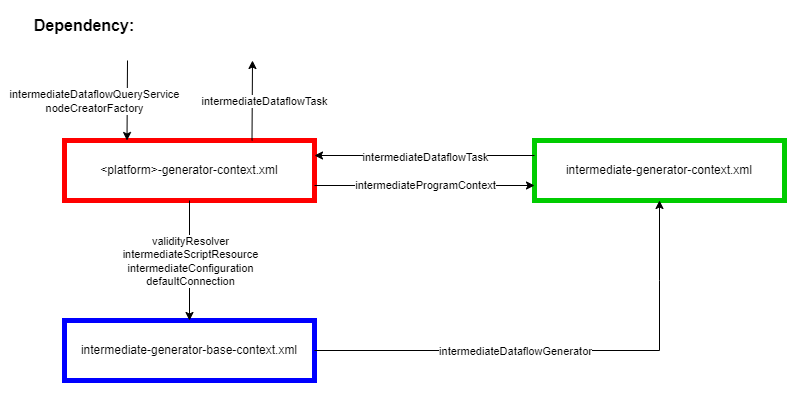
\includegraphics[width=1.0\textwidth]{img/Intermediate Dataflow Generator Configuration-scanner-only dependency.png}
\caption{Dependencies of configurations and their beans}
\label{fig01:ECSbasedesign04}
\end{figure}   

\subsubsection{Composition with Embedded Code Service}
When Embedded Code Service is involved, there needs to be one configuration that satisfies the CLI interfaces and there can be another one that satisfies Code Service needs. Embedded Code Service does not need the CLI interfaces, in fact, they add useless functionality for such use-case, so its best to avoid id. Moreover, in this use-case there could be multiple program configurations passed to Dataflow Generator during its lifecycle so it cannot be defined statically in Spring. To satisfy these needs the platform configurations is split in two parts. First part is configuration of common beans for both use-cases and then there are two specializations that utilize common beans - scanner (CLI) and service specialization.
\begin{figure}[ht]\centering
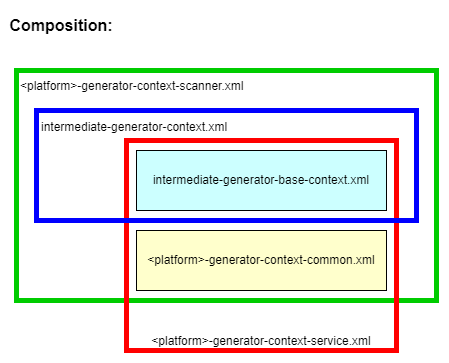
\includegraphics[width=1.0\textwidth]{img/Intermediate Dataflow Generator Configuration-code service-aware composition.png}
\caption{Composition of configurations as they are included in each other}
\label{fig01:ECSbasedesign05}
\end{figure}  
\begin{figure}[ht]\centering
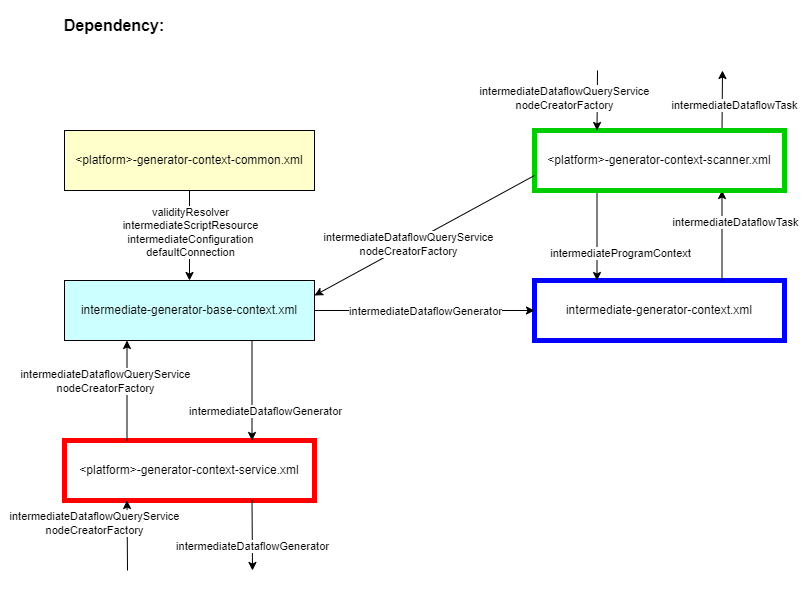
\includegraphics[width=1.0\textwidth]{img/Intermediate Dataflow Generator Configuration-code service-aware dependency.png}
\caption{Dependencies of configurations and their beans}
\label{fig01:ECSbasedesign06}
\end{figure} 




